%%%%%%%%%%%%%%%%%%%%%%%%%%%%%%%%%%%%%%%%%
% Beamer Presentation
% LaTeX Template
% Version 1.0 (10/11/12)
%
% This template has been downloaded from:
% http://www.LaTeXTemplates.com
%
% License:
% CC BY-NC-SA 3.0 (http://creativecommons.org/licenses/by-nc-sa/3.0/)
%
%%%%%%%%%%%%%%%%%%%%%%%%%%%%%%%%%%%%%%%%%

%----------------------------------------------------------------------------------------
%	PACKAGES AND THEMES
%----------------------------------------------------------------------------------------

\documentclass[UTF8,aspectratio=169,14pt]{ctexbeamer}

\usepackage{hyperref}
\hypersetup{
	colorlinks=true,
	linkcolor=red,
	anchorcolor=blue,
	citecolor=green
}

\mode<presentation> {
	
	% The Beamer class comes with a number of default slide themes
	% which change the colors and layouts of slides. Below this is a list
	% of all the themes, uncomment each in turn to see what they look like.
	
	%\usetheme{default}
	%\usetheme{AnnArbor}
	%\usetheme{Antibes}
	%\usetheme{Bergen}
	%\usetheme{Berkeley}
	%\usetheme{Berlin}
	%\usetheme{Boadilla}
	%\usetheme{CambridgeUS}
	%\usetheme{Copenhagen}
	%\usetheme{Darmstadt}
	%\usetheme{Dresden}
	%\usetheme{Frankfurt}
	%\usetheme{Goettingen}
	%\usetheme{Hannover}
	%\usetheme{Ilmenau}
	%\usetheme{JuanLesPins}
	%\usetheme{Luebeck}
	\usetheme{Madrid}
	%\usetheme{Malmoe}
	%\usetheme{Marburg}
	%\usetheme{Montpellier}
	%\usetheme{PaloAlto}
	%\usetheme{Pittsburgh}
	%\usetheme{Rochester}
	%\usetheme{Singapore}
	%\usetheme{Szeged}
	%\usetheme{Warsaw}
	
	% As well as themes, the Beamer class has a number of color themes
	% for any slide theme. Uncomment each of these in turn to see how it
	% changes the colors of your current slide theme.
	
	%\usecolortheme{albatross}
	%\usecolortheme{beaver}
	%\usecolortheme{beetle}
	%\usecolortheme{crane}
	%\usecolortheme{dolphin}
	%\usecolortheme{dove}
	%\usecolortheme{fly}
	%\usecolortheme{lily}
	%\usecolortheme{orchid}
	%\usecolortheme{rose}
	%\usecolortheme{seagull}
	%\usecolortheme{seahorse}
	%\usecolortheme{whale}
	%\usecolortheme{wolverine}
	
	%\setbeamertemplate{footline} % To remove the footer line in all slides uncomment this line
	%\setbeamertemplate{footline}[page number] % To replace the footer line in all slides with a simple slide count uncomment this line
	
	%\setbeamertemplate{navigation symbols}{} % To remove the navigation symbols from the bottom of all slides uncomment this line
}

\usepackage{graphicx} % Allows including images
\graphicspath{{./figs/}}
\usepackage{booktabs} % Allows the use of \toprule, \midrule and \bottomrule in tables
\usepackage{longtable}
\usepackage{listings}
\usepackage{xcolor}
\lstset{numbers=left, %设置行号位置
	numberstyle=\tiny, %设置行号大小
	keywordstyle=\color{blue}, %设置关键字颜色
	commentstyle=\color[cmyk]{1,0,1,0}, %设置注释颜色
	frame=single, %设置边框格式
	escapeinside=``, %逃逸字符(1左面的键),用于显示中文
	%breaklines, %自动折行
	extendedchars=false, %解决代码跨页时,章节标题,页眉等汉字不显示的问题
	xleftmargin=2em,xrightmargin=2em, aboveskip=1em, %设置边距
	tabsize=4, %设置tab空格数
	showspaces=false %不显示空格
}
% Fonts
% \usepackage{libertine}
% \setmonofont{Courier}
\setCJKsansfont[ItalicFont=Noto Serif CJK SC Black, BoldFont=Noto Sans CJK SC Black]{Noto Sans CJK SC}

%\def\imagepath{./resources/graphics}
%\usepackage[imagepath=\imagepath]{ditaa}
%\graphicspath{ {\imagepath/} }


%\usepackage{pgfpages}
%\setbeameroption{show notes on second screen}
%%----------------------------------------------------------------------------------------
%	TITLE PAGE
%----------------------------------------------------------------------------------------

\title[第10讲]{第十讲:进程和线程控制} % The short title appears at the bottom of every slide, the full title is only on the title page
\subtitle{第2节:rCore进程管理}
\author{向勇、陈渝、李国良} % Your name
\institute[清华大学] % Your institution as it will appear on the bottom of every slide, may be shorthand to save space
{
	清华大学计算机系 \\ % Your institution for the title page
	\medskip
	\textit{xyong,yuchen,liguoliang@tsinghua.edu.cn} % Your email address
}
\date{\today} % Date, can be changed to a custom date


\begin{document}
%----------------------------------------------
\begin{frame}
\titlepage % Print the title page as the first slide
\end{frame}
%----------------------------------------------
\begin{frame}
\frametitle{提纲} % Table of contents slide, comment this block out to remove it
\tableofcontents % Throughout your presentation, if you choose to use \section{} and \subsection{} commands, these will automatically be printed on this slide as an overview of your presentation
\end{frame}
%----------------------------------------------
%%	PRESENTATION SLIDES
%----------------------------------------------
%------------------------------------------------
\section{第2节:rCore进程管理}% Sections can be created in order to organize your presentation into discrete blocks, all sections and subsections are automatically printed in the table of contents as an overview of the talk
%------------------------------------------------
% ## rCore进程管理
% 
\subsection{rCore进程管理系统调用}
% 
%------------------------------------------------
\begin{frame}[fragile]
    \frametitle{rCore进程管理系统调用\href{https://rcore-os.github.io/rCore-Tutorial-Book-v3/chapter5/1process.html\#fork}{`fork`}}
    内核会创建一个子进程
    \begin{itemize}
        \item 子进程和调用 `fork` 父的进程在返回用户态时的状态几乎完全相同
        \item 为子进程创建一个和父进程几乎完全相同的应用地址空间。
        \item 父子进程的系统调用返回值`a0` 寄存器内容不同
    \end{itemize}
% 
	\begin{figure}
		\centering
		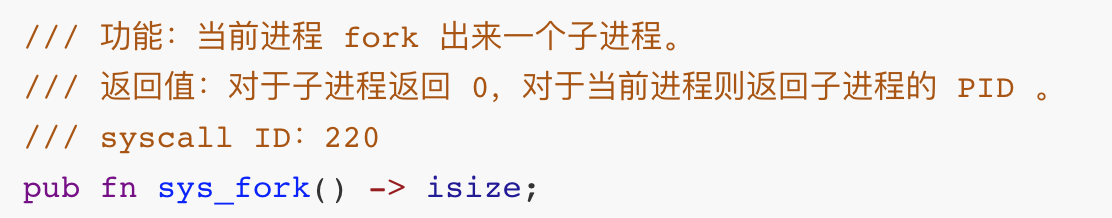
\includegraphics[width=0.9\linewidth]{figs/fork.png}
%		\caption{fork}
	\end{figure}



% 
\end{frame}
%------------------------------------------------
\begin{frame}[fragile]
    \frametitle{rCore进程管理系统调用\href{https://rcore-os.github.io/rCore-Tutorial-Book-v3/chapter5/1process.html\#waitpid}{`waitpid`}}
    \begin{itemize}
        \item 进程通过 `exit` 系统调用退出后,无法立即全部地回收所占用资源
    \begin{itemize}
        \item 内核栈
    \end{itemize}
        \item 父进程通过 `waitpid` 系统调来获取子进程的返回状态并回收所占据的全部资源,从而彻底销毁子进程
    \begin{itemize}
        \item 回收子进程的资源并收集它的一些信息
    \end{itemize}
    \end{itemize}
% 
	\begin{figure}
		\centering
		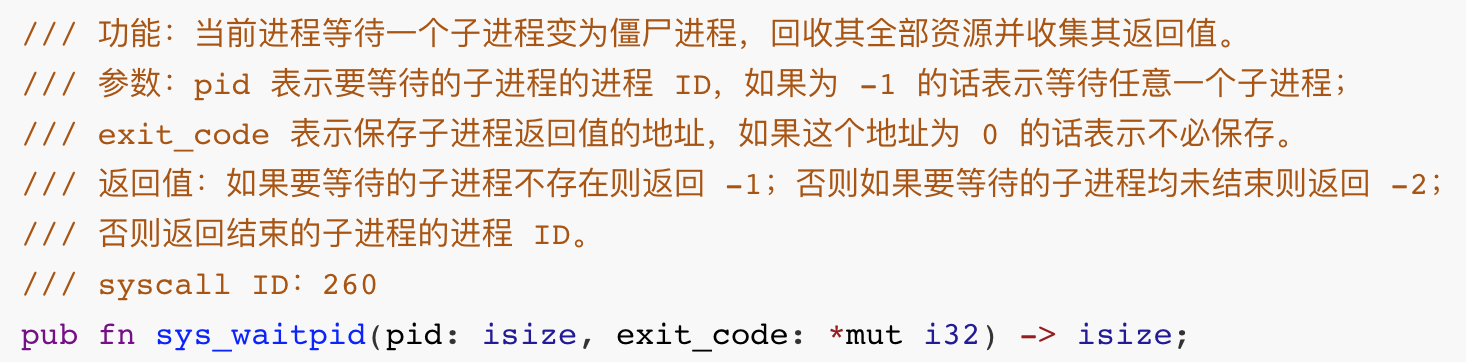
\includegraphics[width=0.9\linewidth]{figs/waitpid.png}
%		\caption{waitpid}
	\end{figure}



% 
\end{frame}
%------------------------------------------------
\begin{frame}[fragile]
    \frametitle{rCore进程管理系统调用\href{https://rcore-os.github.io/rCore-Tutorial-Book-v3/chapter5/1process.html\#exec}{`exec`}}
    执行不同的可执行文件:加载一个新的 ELF 可执行文件替换原有的应用地址空间并开始执行。
    \begin{itemize}
        \item `path` 作为 `\&str` 类型是一个胖指针
    \end{itemize}
% 
	\begin{figure}
		\centering
		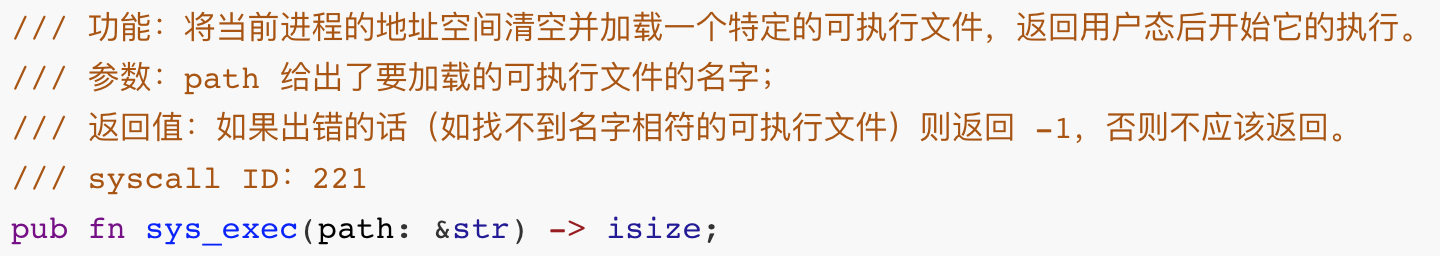
\includegraphics[width=0.75\linewidth]{figs/exec.png}
%		\caption{exec}
	\end{figure}



% 
    \begin{itemize}
        \item 调用方法
    \end{itemize}
% 
	\begin{figure}
		\centering
		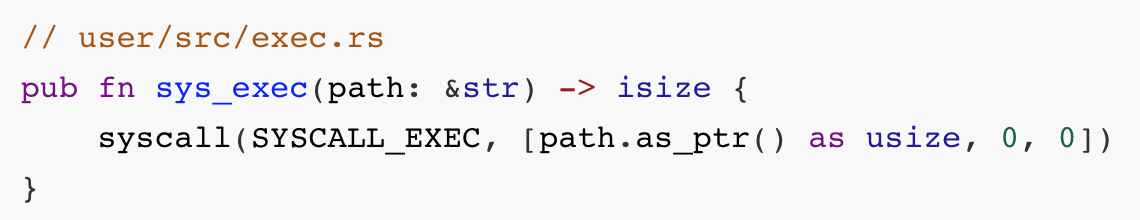
\includegraphics[width=0.65\linewidth]{figs/exec-call.png}
%		\caption{exec-call}
	\end{figure}



% 
\end{frame}
%------------------------------------------------
\begin{frame}[fragile]
    \frametitle{rCore进程管理系统调用`exit`}
    \begin{itemize}
        \item 进程退出:当应用调用 `sys\_exit` 系统调用主动退出或者出错由内核终止之后,会在内核中调用 `exit\_current\_and\_run\_next`函数退出当前任务并切换到下一个。
    \end{itemize}
% 
% 用户初始程序-initproc
% 
% 外壳程序-user_shell
% 
\subsection{进程管理数据结构}
% 
\end{frame}
%------------------------------------------------
\begin{frame}[fragile]
    \frametitle{进程管理数据结构:\href{https://rcore-os.github.io/rCore-Tutorial-Book-v3/chapter5/2core-data-structures.html\#id6}{进程标识符}}
% 
	\begin{figure}
		\centering
		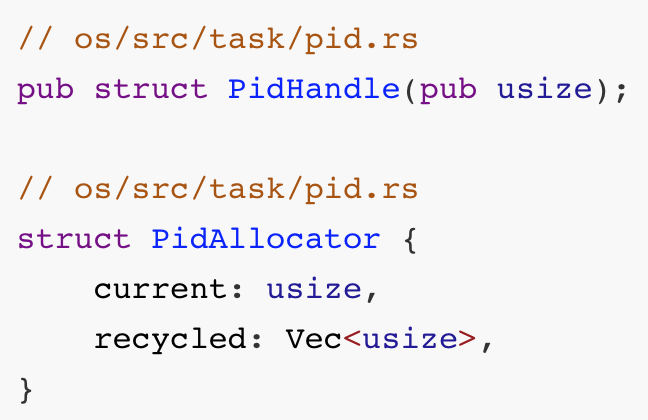
\includegraphics[width=0.6\linewidth]{figs/pid.png}
%		\caption{pid}
	\end{figure}


% 
\end{frame}
%------------------------------------------------
\begin{frame}[fragile]
    \frametitle{进程管理数据结构:内核栈}
% 
	\begin{figure}
		\centering
		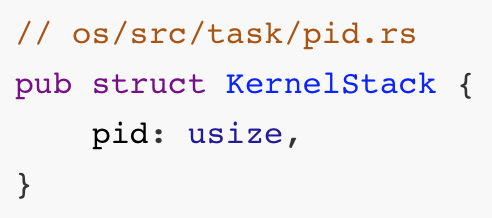
\includegraphics[width=0.5\linewidth]{figs/kernelstack.png}
%		\caption{kernelstack}
	\end{figure}



% 
\end{frame}
%------------------------------------------------
\begin{frame}[fragile]
    \frametitle{进程管理数据结构:\href{https://rcore-os.github.io/rCore-Tutorial-Book-v3/chapter5/2core-data-structures.html\#id7}{进程控制块}}
% 
	\begin{figure}
		\centering
		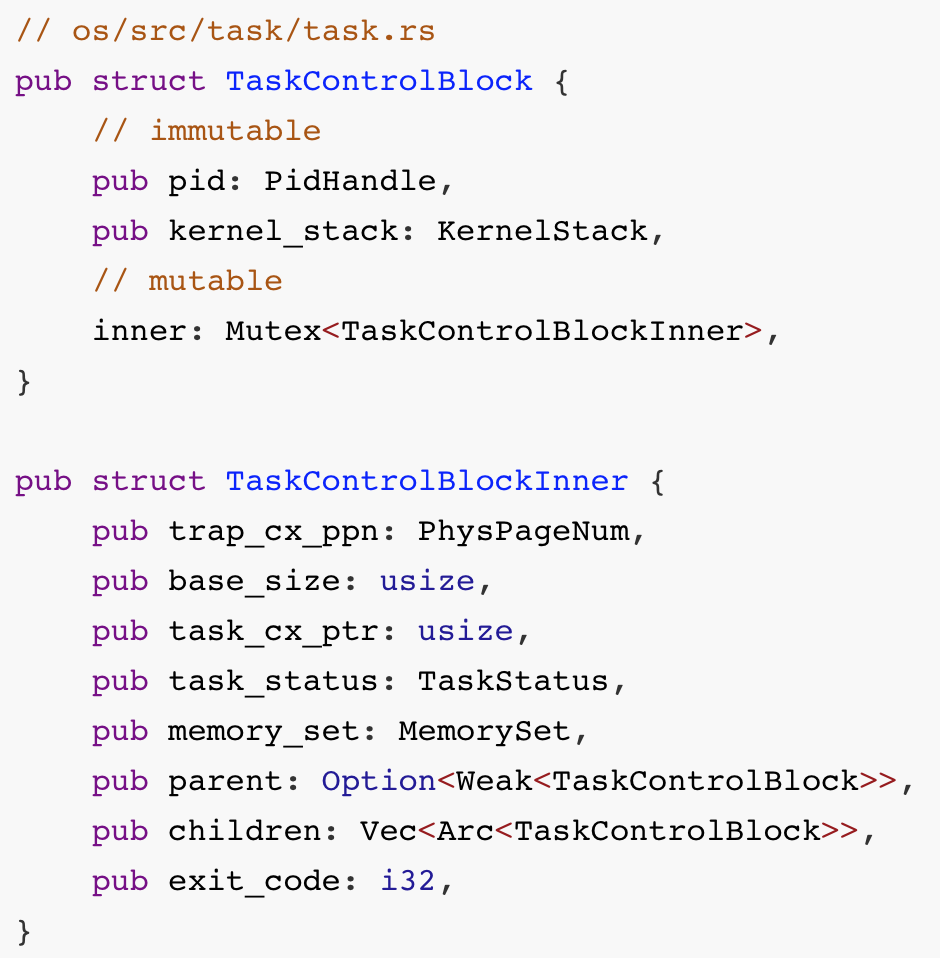
\includegraphics[width=0.45\linewidth]{figs/PCB.png}
%		\caption{PCB}
	\end{figure}



% 
\end{frame}
%------------------------------------------------
\begin{frame}[fragile]
    \frametitle{进程管理数据结构:\href{https://rcore-os.github.io/rCore-Tutorial-Book-v3/chapter5/2core-data-structures.html\#id8}{任务管理器}}
% 
	\begin{figure}
		\centering
		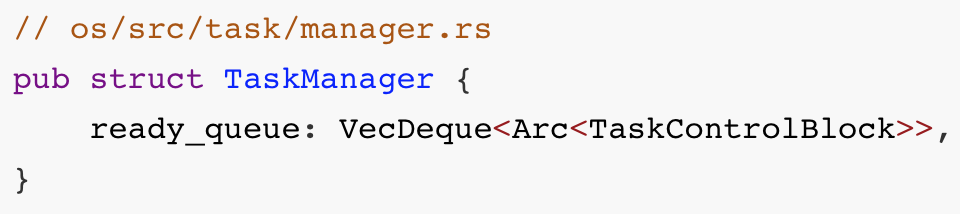
\includegraphics[width=0.7\linewidth]{figs/task.png}
%		\caption{task}
	\end{figure}



% 
\end{frame}
%------------------------------------------------
\begin{frame}[fragile]
    \frametitle{进程管理数据结构:\href{https://rcore-os.github.io/rCore-Tutorial-Book-v3/chapter5/2core-data-structures.html\#id8}{处理器管理结构}}
% 
	\begin{figure}
		\centering
		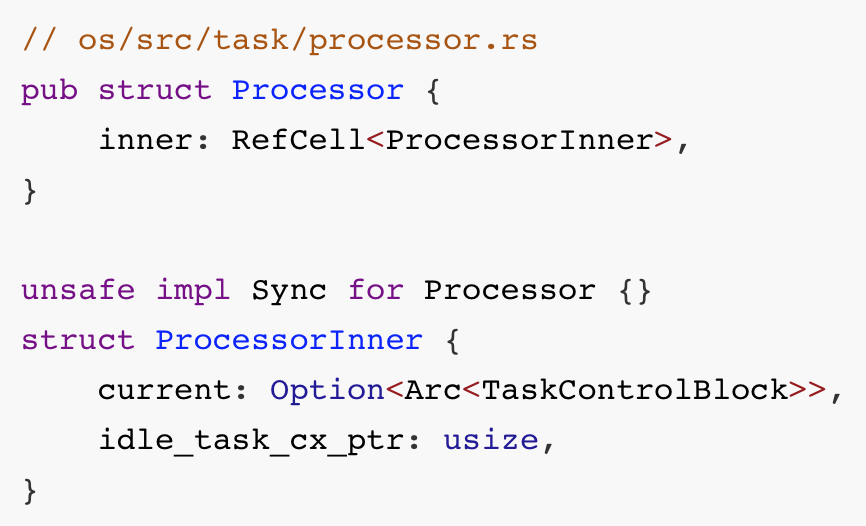
\includegraphics[width=0.7\linewidth]{figs/processor.png}
%		\caption{processor}
	\end{figure}



% 
% 
\end{frame}
%------------------------------------------------
\subsection{任务切换}
%------------------------------------------------
\begin{frame}[fragile]
    \frametitle{\href{https://rcore-os.github.io/rCore-Tutorial-Book-v3/chapter5/2core-data-structures.html\#idle}{任务切换}:\href{https://rcore-os.github.io/rCore_tutorial_doc/chapter6/part2.html}{switch}} 
	\begin{figure}
		\centering
		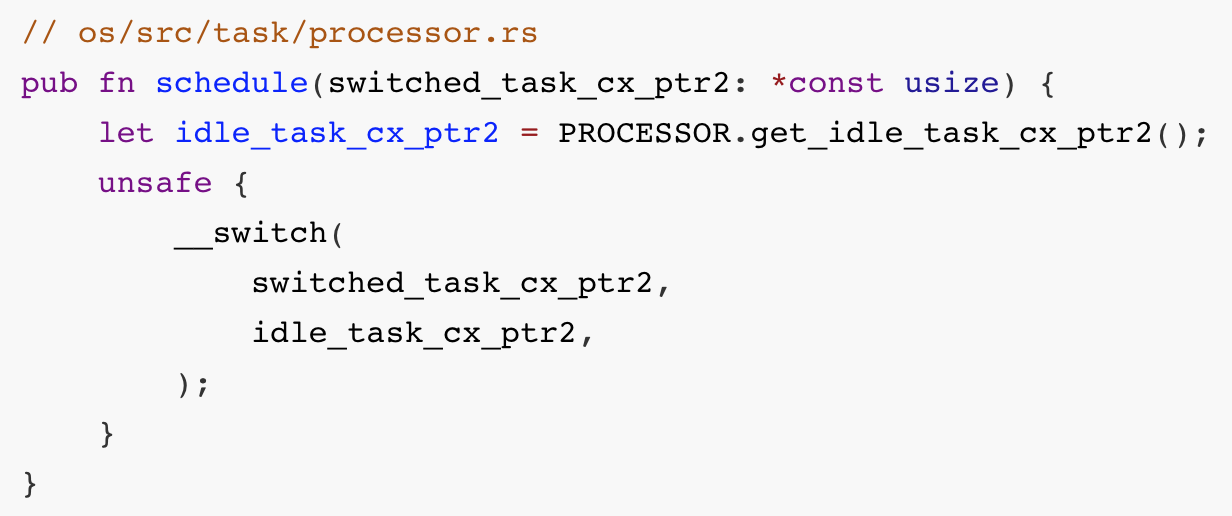
\includegraphics[width=0.7\linewidth]{figs/scheduler.png}
%		\caption{scheduler}
	\end{figure}




\end{frame}
%------------------------------------------------
\end{document}
